\chapter{Implementation}\label{ch:impl}

In this chapter, we discuss the implementation of the individual components
presented in the previous chapter. We also present some shared implementation
features, such as the common request/response protocol used for the
communication between the different components and the coordinator.

\section{Query Library}

As discussed in the previous chapter, queries link against a small wrapper library
which allows submitted Timely programs to participate in our system.
This library performs the initialization of the dataflow computation,
announces its readiness at the coordinator and provides methods for
publishing and subscribing to topics.

For the query to announce itself in the system, the query author must eventually
call the \lstinline{timely_query::execute} function. This function
mirrors Timely's own \lstinline{execute} function in that it performs the execution
of the computation. In contrast to Timely however, our version does not provide
any means to specify the runtime configuration of the execution. This information
is specified by the user at submission time and directly provided to the query library
by its hosting executor. The current implementation of the executor passes
this information down to the query library in environment variables. 

Using this information, the query process connects to the coordinator and registers
itself by providing its identifier and the group of workers it will host. Once
all worker groups have successfully registered themselves at the coordinator,
the coordinator replies with a randomized token which is used to associate
the registered processes with the query.

The initialization of the Timely worker threads and the allocation of the
communication channels among them is by the library done using
\lstinline{time\-ly_\-com\-mu\-ni\-ca\-tion} the same way as it would be done
in a standalone Timely program. For this reason, our query library needs to
translate the information provided by the executor into Timely's own format.

Our query library provides an interface for worker threads to
publish or subscribe to topics. For this reason, every worker thread gets
a handle for the connection to the coordinator. Access to the
publish \& subscribe system is provided through a set of remote
procedure call stubs which are described separately in section~\ref{sec:pubsubimpl}.

\section{Executor}

The current implementation of the executor is relatively simple, it is a
process that spawns child processes on behalf of the coordinator, enabling
the execution of new queries on remote machines.

In order to add a new machine to the cluster, the user has to deploy the executor
binary on the new host, specify the address of the coordinator and then launch
the executor binary. The executor will register itself at the coordinator, which
in turn assigns a unique identifier to the connecting executor. Once connected to the
coordinator, the executor listens for incoming spawn requests. If such a
request arrives, it fetches the binary from the specified source and launches
it as an operating system process. During submission, the user can specifying
command line arguments which are provided to the query binary here as well.

The executor has to inform the spawned binary about its assigned query identifier,
the address of the coordinator and the address of any peer processes. In the
current implementation this is simply done by the executor writing this information
into the environment variables of the spawned query.

The executor currently uses the process spawning functions provided in Rust's standard
library, which at present offer all features we need, and are available on
all supported operating systems. As we will discuss in later chapters,
more sophisticated, platform-specific process control and supervision mechanisms
could be added in the future.

When submitting a new query, the submission must contain an URL to the binary.
The URL scheme determines how the binary is fetched by the executor. In the
current implementation, this can either be a filesystem path directly accessible by the
executor process (e.g. over a shared network folder), or the binary can be provided
over a raw TCP stream. More advanced download schemes can be easily added in
the future.

% TODO talk about the removal of queries
% TODO talk about stdout forwarding

\section{Coordinator}

As the central component of our system, the coordinator performs a rich
set of tasks. These involve handling submission requests to spawn new queries,
but also handling publication and subscription requests from existing queries.
It is the central authority on the current system state, i.e. it maintains
a list of all running queries and executors, but it also tracks all existing
publications and subscriptions. It exposes this information through the catalog.

Because most components interact with the coordinator, its internal implementation
is not without challenges, particularly when dealing with multiple concurrent events.

Before we discuss the details of its implementation, we provide a
brief overview of the internal architecture of the coordinator: To other
components, the coordinator exposes a request/response-based interface on a
predefined networking port. It listens for incoming connections on that port
and then waits for the connected clients to send their requests. Once a request
is received and decoded, it is forwarded to a central request handler.
This request handler contains the central logic of the coordinator, keeps
track of unfulfilled requests, and informs the catalog to announce changes
in the system state.

\subsection{Dealing with Asynchronous Tasks}
Our initial prototype of the coordinator used a multi-threaded approach for dealing
with multiple clients at the same time, and used message passing between threads
to avoid directly exposing shared state. However, many requests handled by
the coordinator require it to wait for external events, and thus a form of
cooperative task management is needed.

We initially used a continuation-passing style for splitting blocking requests into
non-blocking subtasks. However, due to Rust's memory ownership model, we found that
this approach often resulted in manual \emph{stack ripping} \cite{stackmgmt},
which made code both hard to read and inconvenient to write.

This motivated us to re-design the coordinator around a central task dispatch loop, which
allows us to multiplex many asynchronous tasks within the same thread. We decided to adapt
an external library called \lstinline{future-rs} \cite{futuresrs} for this purpose.
It provides an expressive interface for dealing with asynchronous tasks based
on the concept of \emph{futures}. Futures (sometimes called promises, eventuals
or deferred objects) are proxy objects for absent values, which eventually will
be provided through some asynchronous event.
The \lstinline{future-rs} library provides combinators for chaining futures
together or waiting on multiple futures at the same time. Actions on completed
futures are expressed as closures. This approach does not completely eliminate
stack ripping, however the fact that the completion handlers are chained together
allows for much more maintainable and sequentially looking code. Listing~\ref{lst:fnsubscribe}
shows how futures can be used when executing potentially blocking requests.

A unique aspect of the implementation of \lstinline{future-rs} is that its futures
need be polled in order to make progress, instead of proactively being called
by event sources. When a future is polled, it checks if any pending events
have occurred. If so, it dispatches any pending completion handlers. 
It is the users responsibility to ensure that futures are being
polled. This is typically done by registering the future in an event loop,
which will repeatedly wait for events to occur before polling its registered
futures.

\subsubsection{Task Dispatcher}
The \lstinline{future-rs} library itself provides a set of primitives to
create and combine futures. It also provides abstractions for expressing which
events a future is waiting for, and expressing the occurrence of events. It
does however not provide an actual implementation of an event loop. Our implementation
of the coordinator thus provides a simple task dispatcher whose sole purpose it is
to wait for events to occur and poll registered futures accordingly.

To avoid having to pass around a handle to the dispatcher, we store its 
list of pending futures in thread local storage. The public interface consists 
of two free-standing functions, \lstinline{async::spawn} for registering
futures which are to be completed, and \lstinline{async::finish} which initializes
the dispatcher loop and then waits for its termination.
\lstinline{async::finish} accepts an initial future which acts as the root task.
The motivation for the names in this interface comes from the fact that model
each concurrently running task as a chain of futures, basically treating them as
coroutines.

Listing~\ref{lst:coorddispatch} shows an example of this. Our networking layer
models the server socket as a future which yields a stream of incoming connections.
Each connection itself is then maintains a queue for incoming requests, which is
also modeled as a future, allowing the user to specify actions to be taken
once a request is received.

\begin{figure}[htb]
\begin{lstlisting}[caption={[Connection handling at the coordinator]%
Accepting and dispatching incoming connections. The actions specified
in \lstinline{for_each} and \lstinline{map_err} are invoked by the
task dispatcher when the corresponding events (such as new incoming connections,
new incoming requests or errors during request handling) occur.},label={lst:coorddispatch}]
// a future yielding a stream of accepted connections
let listener = network.listen(9189);
// define the action to be executed for each incoming connection
let server = listener.for_each(|connection| {
    ...   
    // this action is invoked for each incoming request
    let client = requests.for_each(move |request| {
        // decode and dispatch request 
        match request.name() {
          "Subscribe" => {
            let (req, resp) = req.decode::<Subscribe>();
            // forward the request to the request handler,
            // which will return a future (see Listing 4.2)
            let subscribe = request_handler
              .subscribe(req)
              .then(|result| Ok(resp.respond(result)));
            // complete this task asynchronously
            async::spawn(subscribe);
          }
          ...
        }
        ...
    }).map_err(|err| {
        // futures can also yield error values
        // which are handeled separately
        error!("failed to dispatch request: {:?}", err)
    });

    // handle client asynchronously
    Ok(async::spawn(client));
});

// drive the event loop to completion
async::finish(server);
\end{lstlisting}
\end{figure}

\begin{figure}[p]
\begin{lstlisting}[caption={[Handler for blocking subscription requests]
Example how a future is created for the subscription request. Depending
on whether it can be served immediately or not, different kinds of futures
are returned. Bookkeeping for still pending requests is done with completion
handles. Upon publication of a requested topic, any pending subscriptions will
be completed by calling \lstinline{lookup.complete()}.},label={lst:fnsubscribe}]
struct RequestHandler {
  catalog: Catalog,
  // list of pending lookups
  lookups: HashMap<String, Vec<Complete<Topic, SubscribeError>>>,
  ...
}

impl RequestHandler {
  pub fn subscribe(&mut self, request: Subscribe)
    -> Box<Future<Item=Topic, Error=SubscribeError>>
  {
    // extract arguments from the request
    let query = request.query.id;
    let name = request.name;
    // first, check if the topic actually exists
    if let Some(topic) = self.catalog.lookup(&name) {
      // if so, insert a new subscription into the catalog
      self.catalog.subscribe(query, topic.id);
      return futures::done(topic).boxed();
    } else if request.blocking {
      // allocate an unresolved future and a completion handle
      let (lookup, result) = promise();

      // to be executed once the topic exists
      let handler = self.handle();
      let result = result.and_then(move |topic| {
        handler.catalog.subscribe(query, topic.id);
        Ok(topic)
      });

      // register the completion handle for pending lookups
      self.lookups.entry(name).or_insert(vec![]).push(lookup);

      return Box::new(result);
    } else {
      // non-blocking subscription request, fail immediately
      let err = SubscribeError::TopicNotFound;
      return futures::failed(err).boxed();
    }
  }
\end{lstlisting}
\end{figure}

\subsection{Maintaining Shared Mutable State}

The nature of the coordinator requires it to mutate its internal state on
behalf of the connected clients. This means that we have to provide each
connection handler with mutable access to the central request handler. 
In addition, we also want to keep track of the requests submitted by
each connection, so we can clean up any associated global state if a connection
disappears.

For this reason, we provide a wrapper type for accessing the methods of the
request handler. For each connection, this proxy maintains a simple list of
identifiers for objects that are conceptually owned by the connection, ensuring that the state is
removed from the catalog once the connection drops. Examples of this are the removal
of disconnected executors from the catalog, or the depublication of topics
owned by crashed queries. The proxy object internally uses Rust's
\lstinline{RefCell<T>} type to dynamically ensure the strict language
rules on shared mutability.

\clearpage

\subsection{Catalog}

The purpose of the catalog is to maintain and expose the current state of the
system. It tracks the addition and removal of executors, queries, topics,
publication and subscriptions and exposes them in collection topics according
to the schema shown in Figure~\ref{fig:model}.

\begin{figure}[htb]
  \centering
    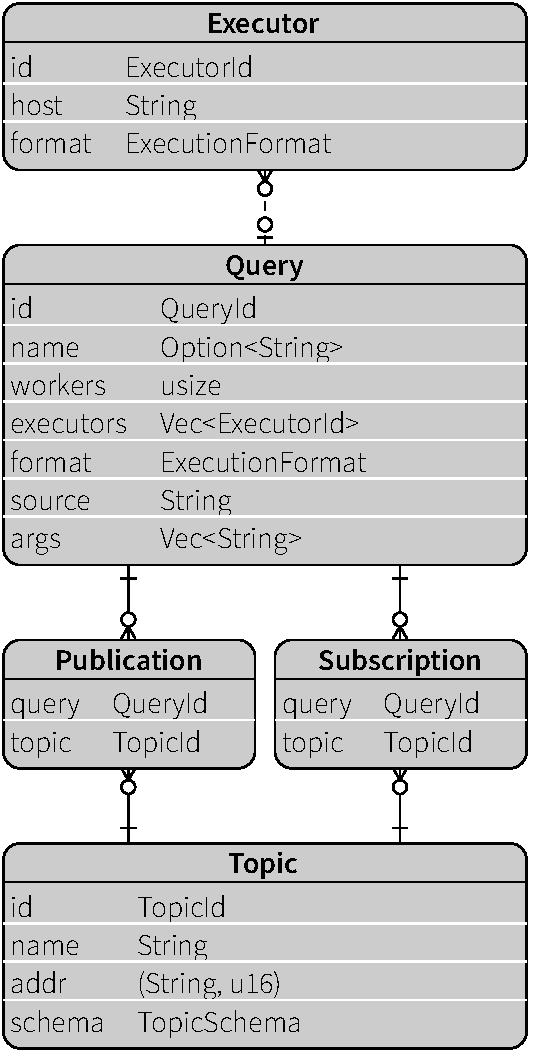
\includegraphics[width=0.5\textwidth]{figures/model}
  \caption[Schema of the catalog]{Schema of the catalog. All five data types
  are published as a collection topic, allowing users to follow state changes
  in the system.}
  \label{fig:model}
\end{figure}

The catalog itself only exposes this data. It is mutated and queried by the
request handler in order to fulfill the submitted requests.


\clearpage
\subsection{Publishers \& Subscribers} \label{sec:pubsubimpl}

The query library exposes the publish and subscribe functionality. The following
API is used for publishing and subscribing to Timely streams.

\begin{figure}[htb]
\begin{lstlisting}[caption={[Publish \& subscribe interface]
The interface for publishing and subscribing Timely streams.
The \lstinline{NonStatic} bounds on the data and timestamp
parameters are required for safe serialization described in \ref{sec:serialization}.
}]
pub struct Coordinator {
  /* hidden handle to request queue */
}

impl Coordinator {
  pub fn publish<S, D>(&self, name: &str, stream: &Stream<S, D>,
    part: Partition) -> Result<Stream<S, D>, PublicationError>
      where D: Data + NonStatic, 
            S: Scope,
            S::Timestamp: NonStatic;

  pub fn subscribe<T, D>(&self, name: &str, cap: Capability<T>) 
    -> Result<TimelySubscription<T, D>, SubscriptionError>
      where T: Timestamp + NonStatic, 
            D: Data + NonStatic;
}
\end{lstlisting}
\end{figure}

\subsubsection{Publisher}

The \lstinline{publish} function takes a direct reference to a Timely
\lstinline{Stream<S, D>}. These stream handles, which are only available during
the dataflow graph construction phase, allow us to instantiate our own publish
operator on the stream.  The instantiated publish operator will push its
incoming data as well as its current frontier to any subscribers. 

Once the operator is inserted into the dataflow graph, the \lstinline{publish}
stub issues a registration request to the coordinator, which will result in the
creation of a topic for other queries to subscribe to.

The partitioning argument on the API specifies whether all streams
shall be merged into a single topic, of if every worker publishes its own stream.
Merging of the stream is done using Timely's partitioning functions. 
In the second case, the identifier of the publishing worker is appended to the
name of the topic. 

\vspace{5em}

\begin{figure}[h!]
\begin{lstlisting}[caption={
Publishing partitioned topics.
}]
timely_query::execute(|root, coord| {
    root.scoped::<u64, _, _>(|scope| {
        let i = scope.index();
        let numbers = (i*100..(i+1)*100).to_stream(scope);

        // results in `n` topics:
        //    "numbers.0", "numbers.1", .., "numbers.n"
        coord.publish("numbers", &numbers, Partition::PerWorker)
             .expect("failed to publish topic");

        // filtering performed by each worker in parallel
        let primes = numbers.filter(|x| x.is_prime());

        // results in a single merged topic called "primes",
        // published by worker with index 0
        coord.publish("primes", &primes, Partition::Merge)
             .expect("failed to publish topic");
    });
})
\end{lstlisting}
\end{figure}

\paragraph{Collection Publisher}

In addition to the stream publisher, we also provide the so called collection
publisher. It has a similar interface for publishing, but it requires the
type of the incoming stream to deliver \lstinline{(D, i32)} tuples, where
the integer denotes the amount of elements that have been added or removed from
the collection.

\begin{lstlisting}[caption={[Collection publisher interface]
}]
impl Coordinator {
  pub fn publish_collection<S, D>(&self, name: &str,
    stream: &Stream<S, (D, i32)>, partition: Partition)
    -> Result<Stream<S, (D, i32)>, PublicationError>
      where D: Data + NonStatic, 
            S: Scope,
            S::Timestamp: NonStatic;
}
\end{lstlisting}

Internally, the publisher maintains a copy of this collection. This is required
for new subscribers, which must be informed about the contents of the collection
when they connect.

\paragraph{Implementation Details}

Both publishers share the same underlying logic which accepts incoming connections
from subscribers and provides notifications for disconnected clients.

Internally, this logic also make use of the \lstinline{future-rs} library, 
since futures have also been integrated in our networking layer.
Inside the coordinator the polling is done by the task dispatcher. For the futures
inside our publish and subscribe operators however we make use of the fact
that Timely itself also uses polling-based scheduling. Every time the publish operator
is scheduled by Timely, it can poll the networking layer to be informed
about newly accepted or disconnected subscribers.

Note that even though each subscription request is disclosed to the coordinator
by subscribing queries, publishers are not informed by the coordinator about new subscribers. Publishers
see new subscribers only once they connect to the publisher's network socket. 
The information stored in the catalog is only exposed for inspection by the user.
Figure~\ref{fig:pubsubseq} shows hows the sequence for publishing a new topic.

\begin{figure}[htb]
  \centering
    \vspace{1em}
    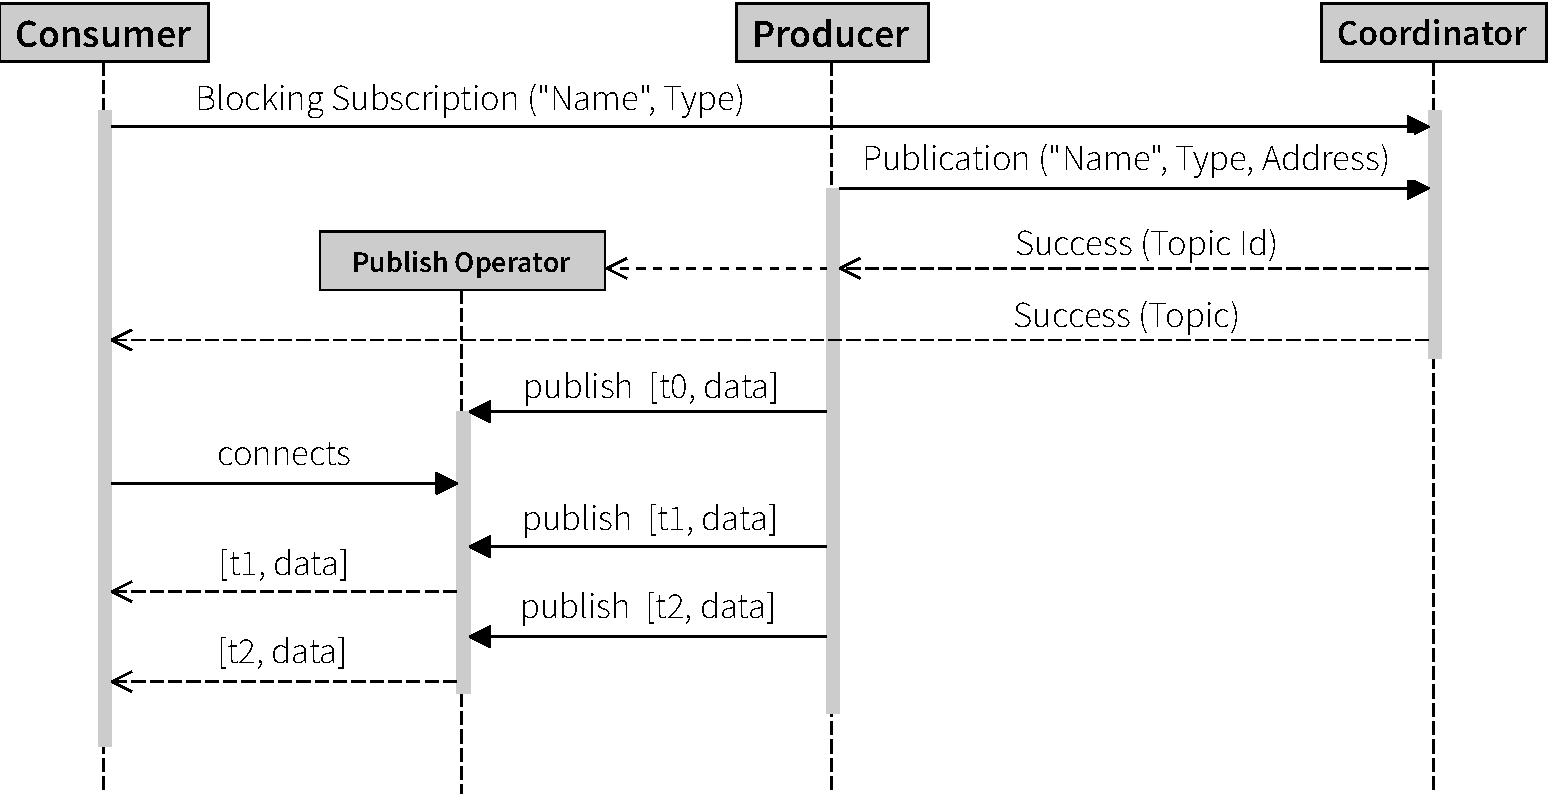
\includegraphics[width=1\textwidth]{figures/pubsubseq}
  \caption[Publish/subscribe sequence diagram]{Sequence diagram for the publish/subscribe procedure. Any data
  produced before the subscriber connects might be lost.}
  \label{fig:pubsubseq}
\end{figure}

\subsubsection{Subscriber}

In contrast to the publisher, the current implementation of the \lstinline{sub\-scribe}
function does not directly instantiate a Timely operator, but returns a subscription
handle which is used to read data from the topic.

There are two reasons for this choice: First, Timely requires that an operator
is instantiated on every worker, such that all instances of the dataflow graph
are identical. However, the amount of topics a query would like to subscribe
to, and the amount of workers it allocates might not match. Thus, the API
quickly becomes complicated, as we would need to provide a way for the 
query author to map topics to operator instances.

Second, Timely's operator contract requires that an operator instance announces
the internal initial capabilities it holds, and, more importantly, the initial
capabilities of its peers. To support this would require some synchronization
between the subscribers, as they have to exchange the initial frontier they
observe at their topic.

Instead, we decided to base our subscription progress tracking on Timely's new
capability handles. The recently added \emph{unordered input operator} allows
a query to feed a computation from data with unordered timestamps. This operator
exposes a root capability for the earliest possible timestamp, allowing the user
to derive capabilities for newer timestamps from old ones. The frontier
is advanced by dropping the capabilities for timestamps for which no more data
is pending.

Based on the progress tracking information delivered by the publisher, the
subscription handle will automatically derive new capabilities for incoming
data and drop old ones if the frontier advances. The user however has to
provide the initial root capability for the input.

\begin{figure}[htb]
\begin{lstlisting}[caption={[Typical use of the subscription handle]
Typical use of the subscription handle. This query subscribes to a single topic of
strings, with \lstinline{u64} being the type of the timestamps.
},label={lst:subhandle}]
timely_query::execute(|root, coord| {

    let (mut input, cap) = root.scoped::<u64, _, _>(|scope| {
        let ((input, cap), stream) = scope.new_unordered_input();
        // stream.operators(..)
        (input, cap)
    });

    let topic = coord.subscribe::<_, String>("example", cap)
                     .expect("failed to subscribe");

    for (time, data) in topic {
        let session = input.session(time);
        session.give_content(&mut Content::Typed(data));
        root.step();
    }
})
\end{lstlisting}
\end{figure}

In queries which use multiple workers, the query author can programmatically
encode which workers subscribe to which topics, as the code outside the
graph generation is allowed to conditionally decide if and how it wants to call
the subscribe function. This functionality is required as there is not
always a one-to-one mapping between published topics and workers at the
subscribing query, and expressing the assignment in arbitrary Rust code
gives the most flexibility to the query author.

Because the root capability can be cloned, this interface also allows the user to
interleave the data from a topic with other data, for example by merging
multiple topics at the input. Our subscription handle implements the
\lstinline{futures-rs} stream interface, allowing the client code to wait for
data from multiple subscriptions at once.

\clearpage
\section{Shared Communications Layer}

For the remainder of this chapter we discuss the networking layer of our system,
which is used by all components to implement their services.

\subsection{Messaging}

Our system consists of potentially many distributed processes. These processes
are running concurrently, are dynamically added and removed from the system
and are communicating with each other. In order to deal with the inherent
complexity of such a system, we adopted an actor-model like approach for our
networking implementation.

Actors in our system include processes like the coordinator, the executors 
and the query processes. But we also treat the publish or subscribe operators
as actors, as they directly interacting with our system.

To support this kind of model, our networking layer also works in terms of
asynchronous messages. In contrast to Timely's own networking layer which also
provides a similar abstraction, we cannot assume a fixed number of components.
In order to establish a connection between two components, one of them has to
take on the role of the server, while the other one acts as a client. Two
queues are allocated per connection on each side: one for incoming messages
and one for outgoing messages. This enables messages to be sent asynchronously
in both directions. Network failures are signaled in the queue for incoming
messages. Currently, Rust's standard library TCP sockets are used as the
underlying transport mechanism, however the system could easily be extended to
support alternative transport layers as well.

\subsection{Request \& Response Messages} \label{sec:reqresp}

While the abstraction of single messages is sufficient for implementing the
mostly unidirectional messaging paradigm of the publish-subscribe implementation,
most other communication in the system follows a request-response pattern,
e.g. any communication with the coordinator.

For this reason, we implemented a request-response multiplexer on
top of the plain message channels. This multiplexer allows both sides to have
multiple requests in flight while waiting for the corresponding responses,
which can be delivered out of order.

In order to differentiate between different kind of requests and also ensure a
well-typed response format, request payloads have to implement the \lstinline{Request}
trait. The associated name is used for decoding, while the associated \lstinline{Success}
and \lstinline{Error} types specify what kind of payloads are valid for the response.
This allows the response for a given request \lstinline{R} to be represented by
Rust's \lstinline{Result<R::Success, R::Error>} type.

\begin{lstlisting}[caption={[Request trait]In order for a type to be used as a
request message, it needs to implement the \lstinline{Request} trait. The name allows
request handlers to differentiate between different types of requests, while the associated
types forces them to issue well-formed responses.
The trait bounds are explained in section \ref{sec:serialization}.}]
pub trait Request: Abomonation + Any + Clone + NonStatic {
    type Success: Abomonation + Any + Clone + NonStatic;
    type Error: Abomonation + Any + Clone + NonStatic;

    fn name() -> &'static str;
}
\end{lstlisting}

\subsection{Serialization} \label{sec:serialization}

For both, the request/response messages as well as messages used in the publish/subscribe
subsystem, we need to serialize the payloads in order to send them over the network.

\subsubsection{Message Buffers}

Incoming and outgoing network data is stored in reference counted message buffers.
This buffer supports multi-part messages, meaning a message contains more than
one serialized object. This is needed for the request/response multiplexer, which
needs to partially decode a message in order to determine to which request it
belongs to. It is also used in the publisher and subscribers, which allows them
to encode and decode the timestamp and the data separately.

Reference counting is an optimization used by publishers, which allows them to
serialize the data only once and share the buffer with all subscribers. Every
outgoing queue to the subscriber only contains a reference to the buffer. Once
the message is written to the subscriber's socket, the reference count is
decreased and the message is deallocated once all subscribers have consumed it.

\subsubsection{Safe Serialization with Abomonation}

Timely itself provides a uses a high-performance serialization library called
Abomonation, implying that all data types sent to a publish operator will be
serializable this way. This makes Abomonation a natural choice as the serialization
format for the messages sent from publishers to subscribers. 

However, Abomonation is neither memory- nor type-safe. There are no safeguards
against deserializing data into an incompatible type, which will result in undefined
behavior. In Timely, such errors are typically avoided since all worker
execute the exact same program code and the streams between workers are
statically typed. In our system however, a publisher might accidentally use
a different version of a library type than the subscriber. Because of this,
we use our own lightweight wrapper around Abomonation. In addition to the raw
serialized bytes, we annotate the buffer with the \lstinline{TypeId} of the
data type. Rust's \lstinline{TypeId} provides an opaque, globally unique
identifier for a given Rust type and its representation. Thus, we can check
if the expected and provided type identifier match before trying to deserialize
a message.

In order for a type to be serialized by our library, it needs to fulfill the
following type bounds: \lstinline{Abomonation + Any + Clone + NonStatic}.

The \lstinline{Any} trait is required to retrieve the type's identifier. The
\lstinline{Clone} trait is used to put deserialized types into the incoming
messages queue and \lstinline{NonStatic} is an auto-trait used to disallow the
creation of eternally valid pointers into temporary buffers. We also take type
alignment rules into consideration when serializing into unaligned buffers. 

\paragraph{Alternative Serialization Formats}

We currently use our safe Abomonation wrapper not only for data in
publish/subscribe system, but also for serializing and deserializing requests
and response messages. This implies that currently all participating components
have to be compiled for the same processor architecture and operating system.

Because of this, our message buffer interface has been designed to use alternative
serialization formats in the future. Besides supporting heterogeneous clusters,
alternative formats might also be useful in the publish/subscribe system:
Schema-based serialization formats would allow subscribers to decode published
data even without static knowledge of its data type.
